
% ----------------------------------------------------------------------
\introduction
\label{sec:intro}
% ----------------------------------------------------------------------

The numerical modelling of past glaciers and ice sheets allows indirect confrontation between glaciological theories and geomorphological reconstructions, challenging the validity of both. In this perspective, the Cordilleran ice sheet in north-western North America is one of the least studied paleo-ice sheets on Earth, where nethertheless significant geomorphological data is available\needref.

To our knowledge, the Cordilleran ice sheet has not been the central target of a numerical modelling study since the one by \citep{roberts-1991}, who focused specifically on its southern margin. However, the Cordilleran ice sheet is often modelled as part of the North-american ice sheet complex\needref, or even of a larger-scale Arctic domain\needref. If these studies reproduce well the magnitude of the North American glaciation at Last Glacial Maximum, they commonly predict excessive ice cover in northern Yukon Territory and Alaska, regions that have not been covered by ice in hundreds of thousands of years\needref.

Here we use a Parallel Ice Sheet Model (PISM) to model the entire Cordilleran ice sheet at the Last Glacial Maximum. We force our model with multiple climate datasets and compare our results to the mapped LGM ice sheet margin. To avoid circular dependance on prescribed ice sheet geometries, we use present-day climate data and given temperature offsets rather than LGM climate model runs.

\begin{figure}[t]
	\vspace*{2mm}
	\begin{center}
		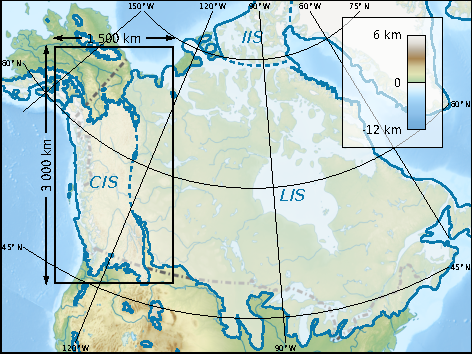
\includegraphics[width=8cm]{cordillera-climate-locmap}
	\end{center}
	\caption{Shaded relief map of northern North America. The frame delimits this study's modelling domain. The outlines of the former ice sheets are from \citet{kleman-etal-2010}. The background map was made with ETOPO1 \citep{data:etopo1} and Natural Earth Data \citep{data:naturalearth}.}
	\label{fig:locmap}
\end{figure}

